\documentclass[myclassdoc,debug]{rjparticle}
%use the following command when typesetting your paper:
% \documentclass{rjparticle}
\usepackage{graphicx}

\title{Extensive Study of the Wobbling Properties in $^{163}$Lu Based on a Parity Symmetry Property} 

\author[1,2,$a$]{Robert Poenaru}

\author[1,3,$b$]{Apolodor Aristotel Raduta}

\affil[1]{``Horia Hulubei'' National R\&D Institute for Physics and Nuclear Engineering,\\
Reactorului 30, RO-077125, P.O.B. MG-6, M\u{a}gurele-Bucharest, Romania
\email[a]{robert.poenaru@drd.unibuc.ro} (corresponding author)}
\affil[1]{``Horia Hulubei'' National R\&D Institute for Physics and Nuclear Engineering,\\
Reactorului 30, RO-077125, P.O.B. MG-6, M\u{a}gurele-Bucharest, Romania}
\affil[2]{Doctoral School of Physics, University of Bucharest, Romania}
\affil[3]{Academy of Romanian Scientists, Bucharest, Romania\\
\email[b]{raduta@nipne.ro}}


\keywords{Wobbling Motion, Nuclear Structure, Parity Symmetry}

\pacs{pacs}

\hyphenation{rjp-ar-ti-cle}

%%%%%%%%%%%%%%%%%%%%%%%%%%%%%%%%%%%%%%%%%%%%%%%%%%%%%%%%%%%%%%%%%%%%%%%%%%%%%%%
%Please, do not remove the following lines!
%%%%%%%%%%%%%%%%%%%%%%%%%%%%%%%%%%%%%%%%%%%%%%%%%%%%%%%%%%%%%%%%%%%%%%%%%%%%%%%
%\RJPVolume{63}{2018}
%\RJPNumber{1-2}
%\RJPPages{}{}
\columntitle{A shorter version of the title to fit one line header of odd pages}
%\date{\today}
%\dedication{}
%\domaintitle{}
%\keywords{}
%\pacs{01.30.-y}
%%%%%%%%%%%%%%%%%%%%%%%%%%%%%%%%%%%%%%%%%%%%%%%%%%%%%%%%%%%%%%%%%%%%%%%%%%%%%%%

\begin{document}
%%%%%%%%%%%%%%%%%%%%%%%%%%%%%%%%%%%%%%%%%%%%%%%%%%%%%%%%%%%%%%%%%%%%%%%%%%%%%%%
%Please, remove these lines when typesetting your document!
%%%%%%%%%%%%%%%%%%%%%%%%%%%%%%%%%%%%%%%%%%%%%%%%%%%%%%%%%%%%%%%%%%%%%%%%%%%%%%%
\lstset{%
basicstyle=\small,
language=[AlLaTeX]TeX,
columns=fullflexible,
%keepspaces=true,
showspaces=true,
showstringspaces=false,
keywordstyle=[2]\ttfamily,
identifierstyle=,
texcsstyle=*\ttfamily,
commentstyle=\color{gray},
string=[s]<>,
morestring=[b]',
stringstyle=\emph,
breaklines=true,
deletekeywords={list},
moretexcs={authnote,keywords,pacs},
}
%%%%%%%%%%%%%%%%%%%%%%%%%%%%%%%%%%%%%%%%%%%%%%%%%%%%%%%%%%%%%%%%%%%%%%%%%%%%%%%
\maketitle
\begin{abstract}
A new interpretation on the wobbling structure in $^{163}$Lu is developed, based on the concept of parity symmetry. It is known that four wobbling bands are experimentally observed in this isotope, where three of them are considered as wobbling phonon excitations (namely $TSD_2$, $TSD_3$, and $TSD_4$) and the yrast band for the ground state (that is TSD1). In the present work, the trial function that is used for obtaining the wobbling spectrum is analyzed in terms of its behavior under the rotation operation. Indeed, due to a specific symmetry to rotations with $\pi$ around the 2-axis of the triaxial system, the parity becomes a good quantum number. As such, the trial function admits solutions with negative parity, which belong to the rotational states in $TSD_4$. A unified description of all the triaxial super-deformed bands in $^{163}$Lu is achieved with the new formalism.
\end{abstract}

\section{Introduction}
Wobbling motion in nuclei was extensively studied in the recent years, and the scientific community finally shed some light on this elusive phenomenon. This kind of collective motion was firstly predicted by Bohr and Mottelson, more than 50 years ago \cite{BMott}.

\section{Theoretical Background}

In a previous work, a complete description of the triaxial characteristics of the Lu isotopes was given, where results for the wobbling energies and transition probabilities were presented \cite{Raduta2018}.

In this paper, the wobbling spectrum is represented. See Figure \ref{tsd_spectrum} for more details.

\begin{figure}[ht]
    \centering
    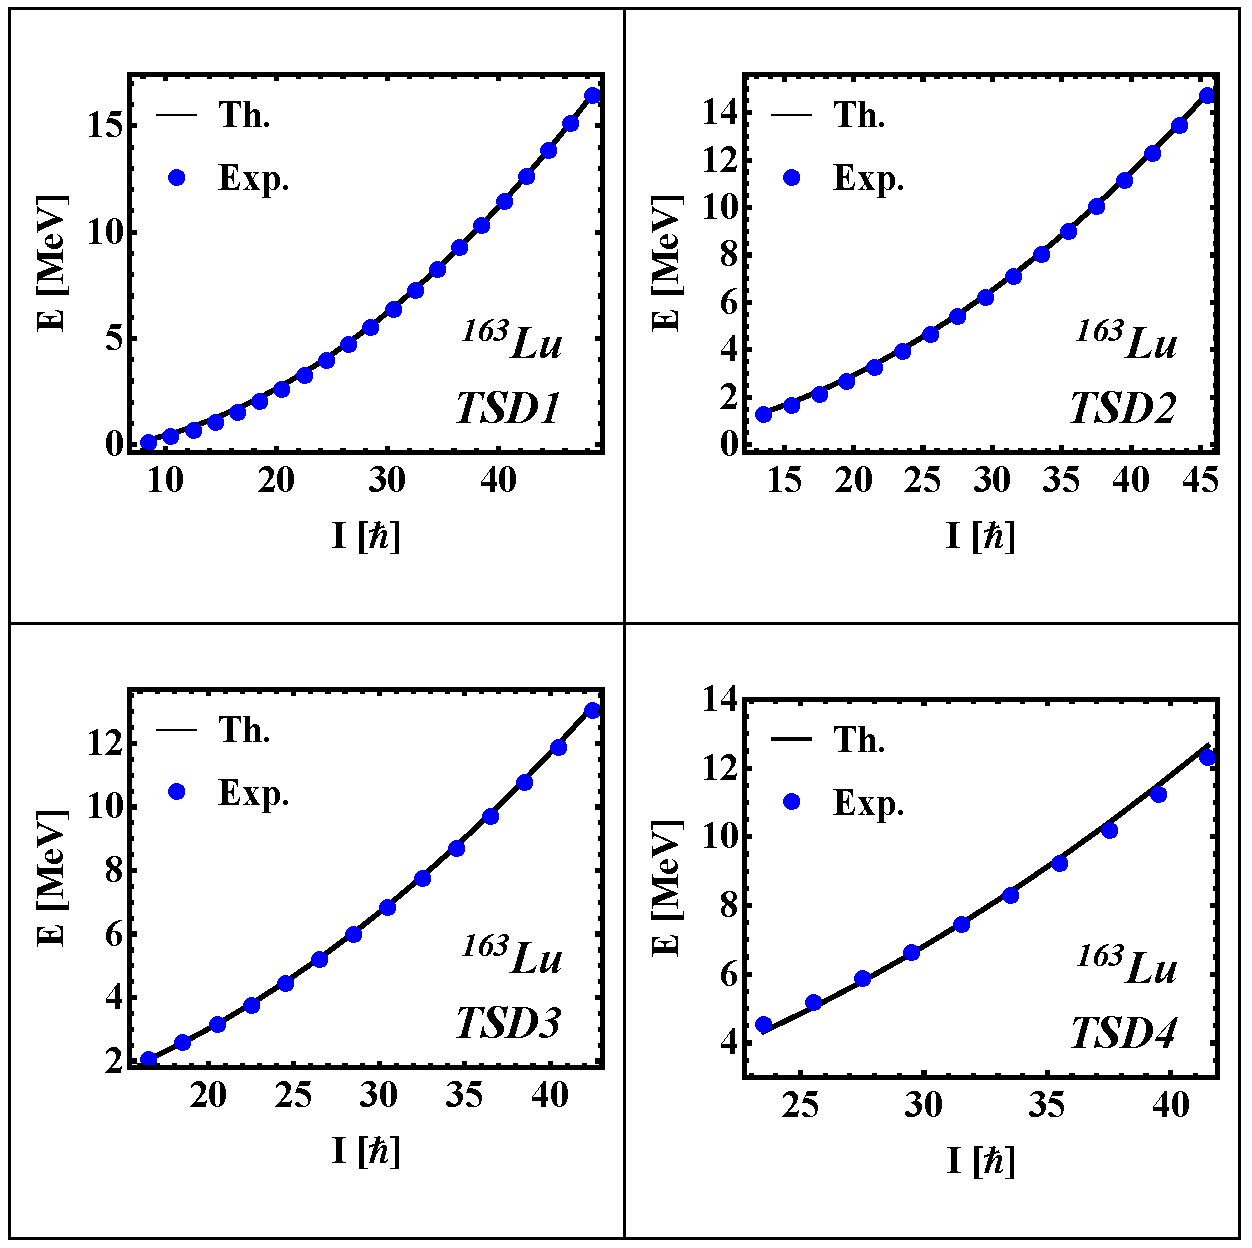
\includegraphics[scale=0.5]{simple-code/figs/ExcitationEnergies_GridView.pdf}
    \caption{The excitation energies for the wobbling spectrum of $^{163}$Lu. Comparison with the available experimental data.}
    \label{tsd_spectrum}
\end{figure}

The contour plots for a state within each of the four bands are properly shown in Figure \ref{contours}.

\begin{figure}[ht]
    \centering
    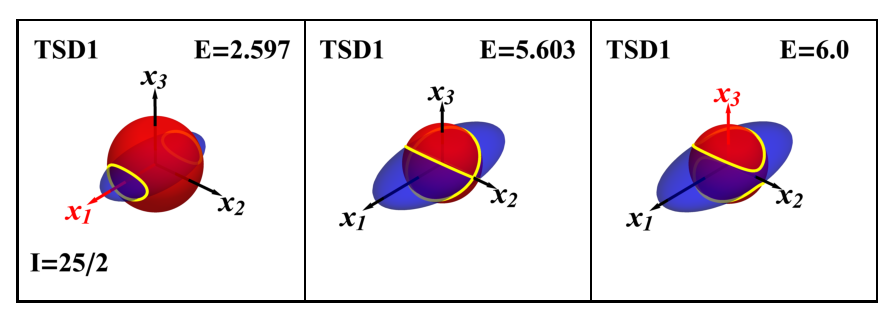
\includegraphics[scale=0.5]{simple-code/figs/tsd1_spin1.eps}
    \caption{The contour plots with the energy function $\mathcal{H}$ of the nucleus, evaluated for the obtained fit parameters.}
    \label{contours}
\end{figure}

\begin{acknowledgement}
We are grateful.
\end{acknowledgement}

\begin{thebibliography}{99}

\bibitem{BMott}A.  Bohr and B.  Mottelson, {\it Nuclear Structure} (Benjamin, Reading, MA, 1975), Vol.  II, Ch.  4. 
\bibitem{Raduta2018}A.  A.  Raduta, R.  Poenaru and Al.  H.  Raduta, J.  Phys.  G: Nucl.  Part.  Phys.  {\bf 45} 105104 (2018). 

\end{thebibliography}


\end{document}